\section{Résolution par Intervalles}
Les méthodes formelles et numériques, bien que performantes par certains aspects, sont rapidement limitées lorsque l'on veut résoudre des problèmes complexes ou que l'on veut pouvoir valider une solution (problème de propagation des erreurs\dots{}). C'est dans ce cadre que la méthode de résolution par intervalles a toute sa place. Construite grâce à l'arithmétique des intervalles, elle utilise aussi des notions apportées par la programmation par contraintes.
 
\subsection{L'Arithmétique des intervalles}
Cette arithmétique permet un calcul sur l'ensemble $\mathbb{I}$ des intervalles à bornes sur $\mathbb{R}$. Les bornes $b1$ et $b2$ de l'intervalle $[b1,b2]$, résultant de tout calcul, sont choisies en prenant un arrondi respectivement inférieur à $b1$ et supérieur à $b2$ de manière à garantir l'exactitude des calculs. L'extension des fonctions aux intervalles, introduite par \textsc{Moore} en 1966, permet une transition à des intervalles grâce à un opérateur d'encadrement. Les opérations élémentaires sont alors réécrites en terme des bornes des intervalles, par exemple : 

\begin{equation}\label{eq2}
\begin{cases}
[a .. b] + [c .. d] = [a + c .. b + d] \\
[a .. b] × [c .. d] = [min(ac, ad, bc, bd) .. max(ac, ad, bc, bd)]
\end{cases}
\end{equation}

Dans le cas d’une fonction non monotone comme le cosinus, on découpe les intervalles en domaines où la fonction est monotone  (\ref{fig:Cos})

\begin{figure}[h] %on ouvre l'environnement figure
  \center
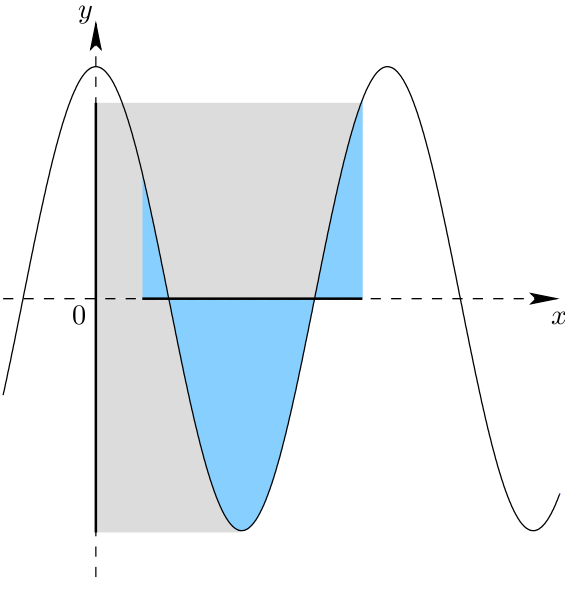
\includegraphics[scale=0.30]{img/cos}
  \caption{Cas de la fonction cosinus} %la légende
 \label{fig:Cos} %la légende
\end{figure} %on ferme l'environnement figure


Une liste non-exhaustive des opérations de cet opérateur est listée dans \cite{Goualard}.



\subsection{Utilisation des intervalles pour la notion de contraintes}
\'Egalement, la méthode de résolution par intervalles utilise des notions de programmation par contraintes. On y retrouve celle de consistance. La consistance consiste à rechercher les valeurs cohérentes dans le domaine des variables pour les contraintes du \textsc{CSP}. Par exemple un \textsc{CSP} est globalement consistant lorsque toutes les valeurs des variables de son domaine appartiennent au moins à une solution. On devine qu'il peut être intéressant pour un \textsc{CSP} de posséder la consistance la plus forte possible. Ainsi les opérations pour la résolution de problèmes seront moins nombreuses. %Cette méthode appliquée au problème d'intersection de deux cercles, illustre les solutions de la manière suivante   

%~ \begin{figure}[ht!] %on ouvre l'environnement figure
  %~ \center
%~ 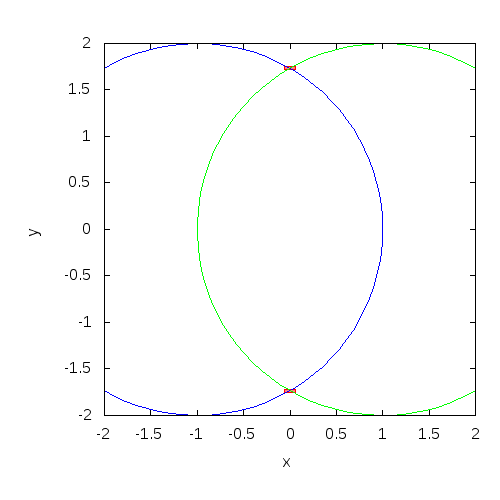
\includegraphics[scale=0.55]{img/circle-circle}
  %~ \caption{Intersection de deux cercles} %la légende
 %~ \label{fig:Deuxcerlces} %la légende	
%\end{figure} %on ferme l'environnement figure
On visualise ici que les solution sont encadrées par des \og boîtes \fg{} rouges, et non réduites à des points. 

Dans le cas du problème \ref{eq2}, il serait possible d'avoir des solutions différentes selon la consistance choisie. Avec une hull-consistance, nous obtiendrions une boite contenant les deux solutions mais aussi une bonne partie de l'intersection des deux cercles. La \emph{3B-consistance} est une méthode plus puissante. Cette méthode vérifie, à l'instanciation de deux variables, vérifie localement toutes les contraintes. Une illustration des différences entre ces méthodes est proposée sur la figure \ref{fig:3Bconst}. Le problème résolu est celui de l'intersection de deux disques.
\begin{figure}[ht!] %on ouvre l'environnement figure
  \center
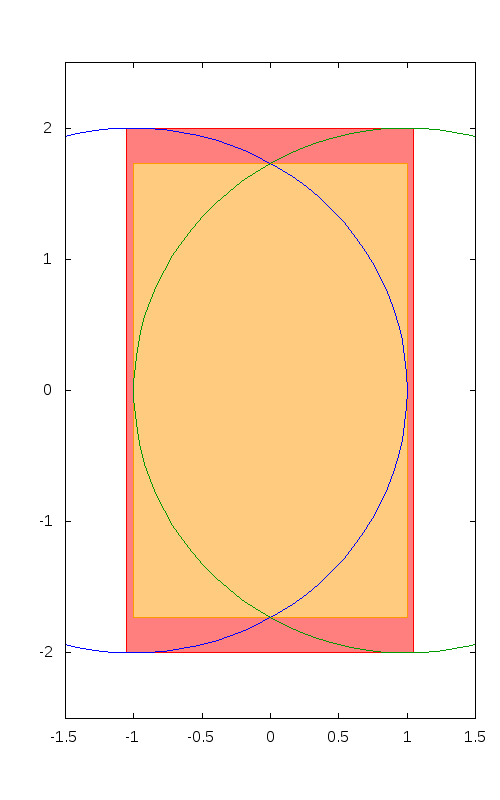
\includegraphics[scale=0.35]{img/disk-disk2}
  \caption{Comparaison graphique entre la Hull-consistance (rouge) et la 3B-consistance (orange)} %la légende
 \label{fig:3Bconst} %la légende	
\end{figure} %on ferme l'environnement figure


\subsection{Exemples d'application}

La précision de la méthode attirent le monde industriel. Notamment les applications composées de contraintes géométriques comme la robotique. La figure \ref{fig:rob} illustre un robot avec deux points d'encrage ($P_1$ et $P_2$) possédant chacun un bras rotatif de longueurs respectives [$L_1$] et [$L_2$] et orientés respectivement par les angles $\alpha_1$ et $\alpha_2$. Ces bras sont composés de pistons permettant d'ajuster leurs longueurs. Ainsi leurs longueurs de bras sont comprises respectivement entre $[L_{1min} \dots L_{1max}]$ et $[L_{2min} \dots L_{2max}]$ et les angles entre $[\alpha_{1min} \dots \alpha_{1max}]$ et $[\alpha_{2min} \dots \alpha_{2max}]$.  

\begin{figure}[h] %on ouvre l'environnement figure
  \center
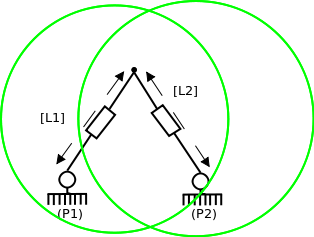
\includegraphics[scale=0.80]{img/robot2}
  \caption{Exemples d'application dans la robotique} %la légende
 \label{fig:rob} %la légende
\end{figure} %on ferme l'environnement figure
L'objectif est de connaitre l'ensemble des emplacements possibles pour la main du robots en fonction des paramètres donnés ci-dessus. Dans le cas de la figure \ref{fig:rob}, on peut considérer que les $L_{imin}$ sont nulles et que les bras puissent effectuer des rotations de $360 \degres$. Ainsi le problème consiste à retrouver l'intersection de deux disques. 

  Par ailleurs, ces méthodes intéressent régulièrement les industriels. On retrouve en effet dans \cite{Schichl}, les détails d'applications dans le secteur de la chimie industrielle mais aussi dans celui de la biologie avec une étude sur les protéines. La science fondamentale met aussi en application ces outils. C'est le cas en mathématique par exemple de problèmes tel que la conjecture de \textsc{Kepler} ou encore le  maximum de clique.

\clearpage
